\begin{figure}[!h]
\centering
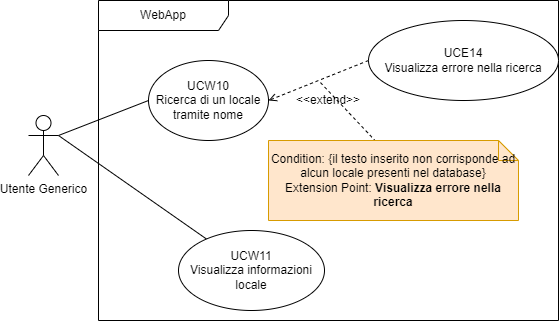
\includegraphics[scale=0.5]{UC_images/UCW10-11.png} 
\caption{UCW10 – Ricerca di un locale tramite nome}
\end{figure}

\subsection{UCW10 – Ricerca di un locale tramite nome}
\begin{itemize}
    \item \textbf{Descrizione}: L'utente generico effettua la ricerca di un locale tramite il suo nome.
    \item \textbf{Attore primario}: Utente generico.
    \item \textbf{Precondizione}: L'utente si trova all’interno della piattaforma Sweeat.
    \item \textbf{Postcondizione}: Viene visualizzato la lista dei locali ricercati.
    \item \textbf{Scenario principale}: 
    \begin{enumerate}
        \item L’utente va nella barra di ricerca della piattaforma;
        \item L’utente digita il nome del locale da cercare;
        \item L’utente clicca sul bottone di ricerca;
    \end{enumerate}
    \item \textbf{Estensioni}:
    \begin{itemize}
        \item Nel caso in cui l’utente l’utente inserisce un testo non corrispondente a nessun locale presente nel database
	\begin{enumerate}  
		\item L’utente va nella barra di ricerca della piattaforma;
        \item L’utente digita il nome del locale da cercare;
        \item L’utente clicca sul bottone di ricerca; 
        \item Viene mostrato un messaggio d'errore, nel caso non sia presente alcun locale simile al locale ricercato(UCE14 §).
    	%Visualizzazione di un messaggio informando che non è presente nessun locale con tale nome e viene suggerita una lista di locali simili a quello ricercato.   
    \end{enumerate}
    \end{itemize}    
\end{itemize}

\subsection{UCW11 – Visualizza informazioni locale}
\begin{center}
\end{center}
\begin{itemize}
    \item \textbf{Descrizione}: L'utente generico visualizza le informazioni di un locale.
    \item \textbf{Attore primario}: Utente generico.
    \item \textbf{Precondizione}: L'utente ha svolto la funzione di ricerca di un locale o sta visualizzando la classifica dei locali.
    \item \textbf{Postcondizione}: Vengono visualizzate le informazioni di un locale.    
    \item \textbf{Scenario principale}: 
    \begin{enumerate}
    \item L'utente seleziona un locale tra quelli presenti nella lista;
    \item Il sistema mostrerà all'utente le informazioni relative al locale scelto.
    \end{enumerate}
\end{itemize}
